
Question 1.2:\\	
\textsl{Provide at least one visualization which supports the claim that within each of the three types, there are numerous possible sub-types for a cell. In your visualization, highlight which of the three main types these sub-types belong to. Again, explain how your visualization supports the claim.}\\

Answer:\\
The "elbow" plot indicates, that the data could be clustered in 3 clusters (see figure \ref{fig:elbow_plot}). But because of a smooth transition towards a larger number of clusters, there could be as well multiple sub-clusters, as the scientist suggests.\\

\begin{figure}[h]
	\centering
	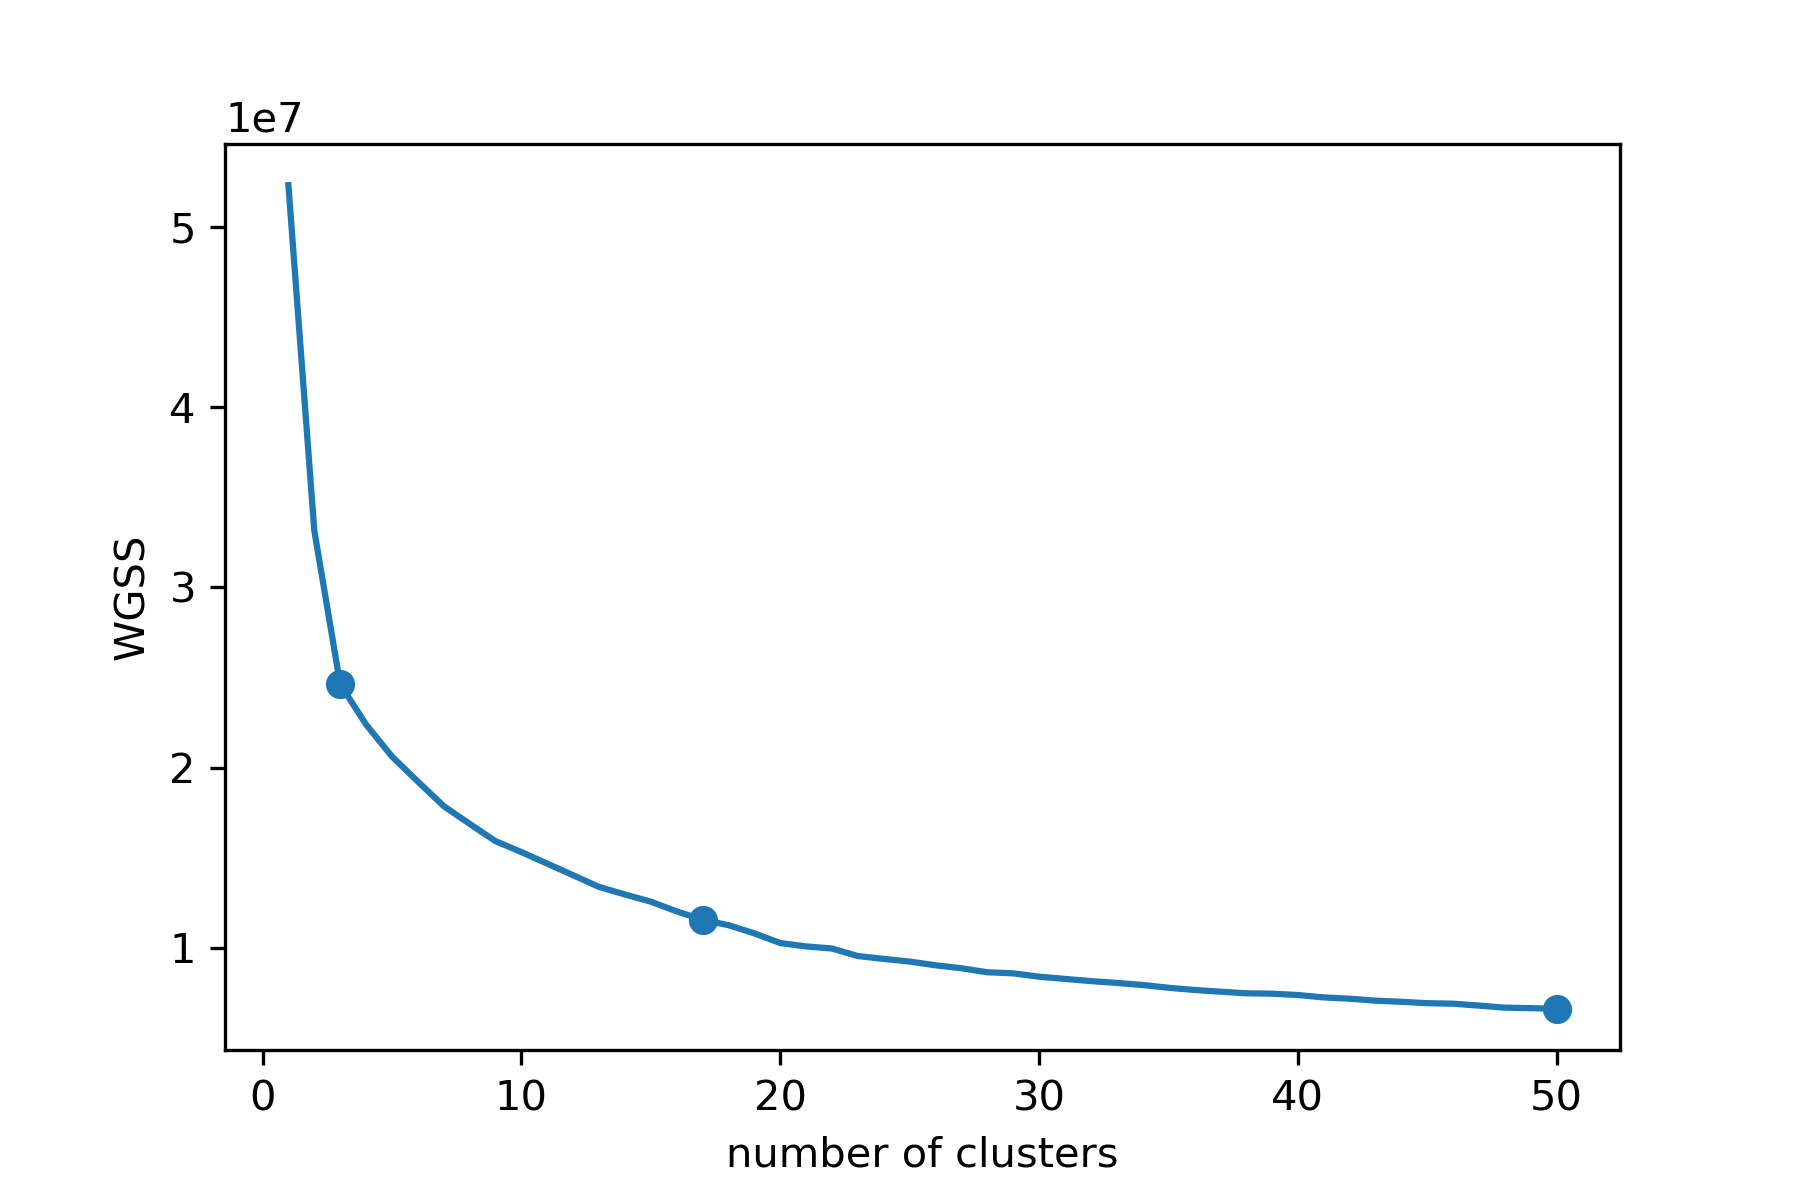
\includegraphics[width=0.5\linewidth]{problem_02/elbow_plot}
	\caption{"Elbow" plot (WGSS (K-Means inertia) over number of clusters)}
	\label{fig:elbow_plot}
\end{figure}

By reducing the perplexity of the T-SNE function to 100 the sub-clusters are moved apart, which makes the distinction easier (see figure \ref{fig:number_clusters_TSNE}). For demonstration purposes, 3 different number of clusters indicate that there are multiple sub-clusters. These might correspond to different cell types within the 3 main types. But there is a compromise between differentiation and merging of clusters. Big groups tend to melt together, whereas smaller groups are better distinguished with an increasing number of clusters. To find the "sweet spot", it is recommended to compare this model with labels of the real data set.\\

\begin{figure}[h]
	\centering
	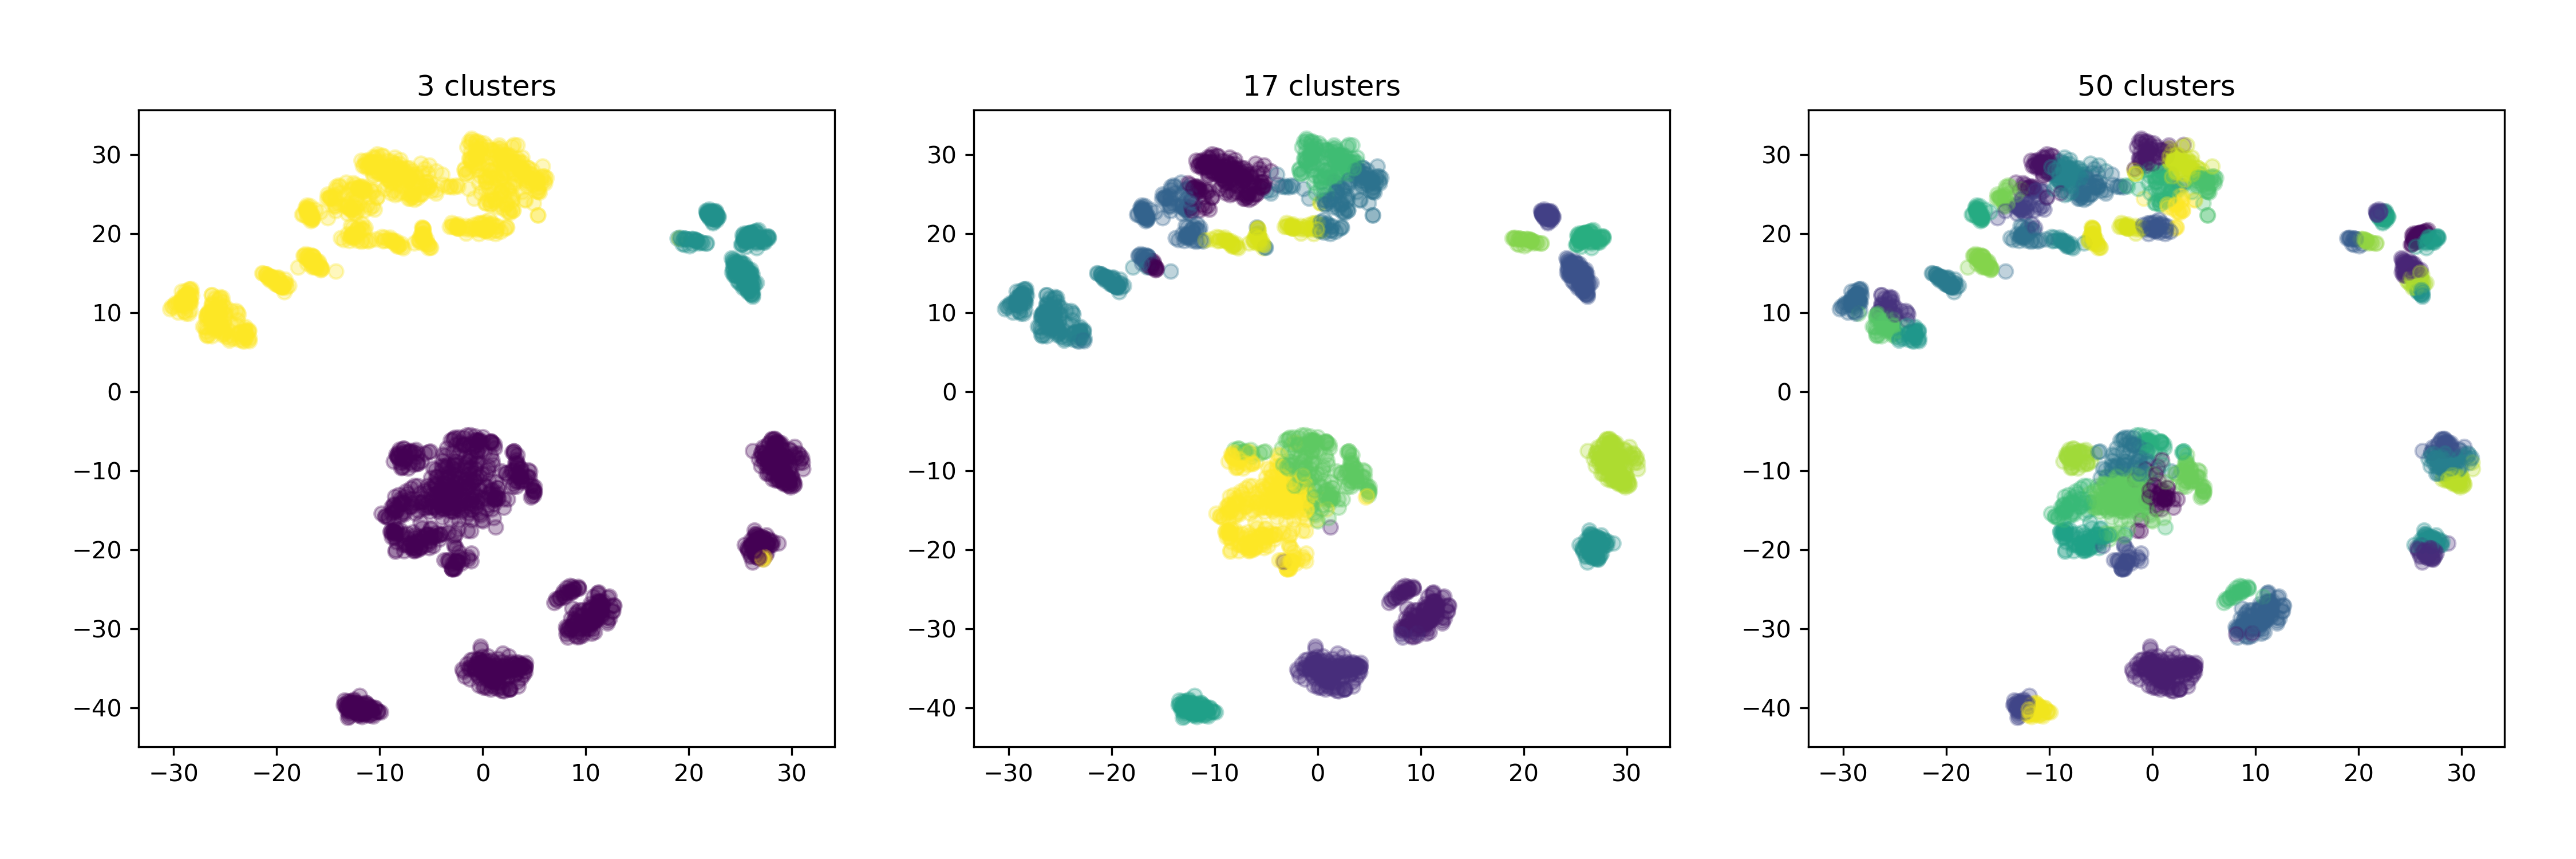
\includegraphics[width=1\linewidth]{problem_02/number_clusters_TSNE}
	\caption{Different number of clusters for T-SNE (perplexity = 100)}
	\label{fig:number_clusters_TSNE}
\end{figure}

To get further information, about how well the data was clustered, we could use a silhouette plot. The better the model represents the data, the higher the silhouette coefficient gets. This step is skipped at this point and done in the following part.\\